\documentclass[tikz,border=10pt]{standalone}
\begin{document}
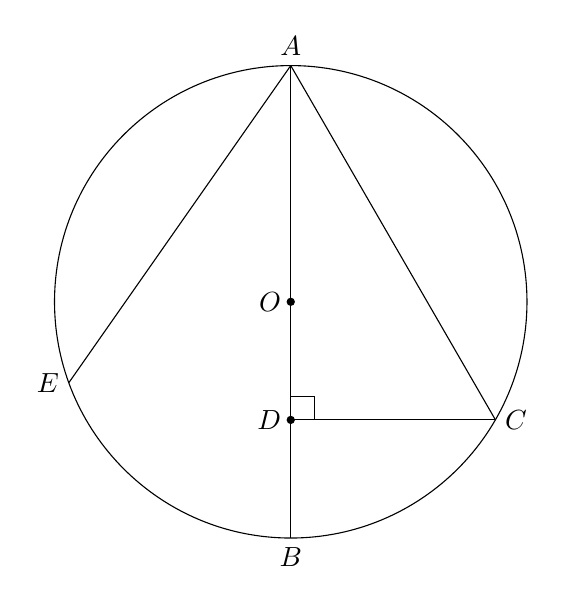
\begin{tikzpicture}
    \coordinate (O) at (0,0);
    \coordinate (A) at (0,3);
    \coordinate (B) at (0,-3);
    \coordinate (D) at (0,-1.5);
    \coordinate (C) at (2.6,-1.5);
    \coordinate (E) at (-2.82,-1.03);

    \draw (O) circle (3);
    \draw (A) -- (B);
    \draw (A) -- (C);
    \draw (A) -- (E);
    \draw (D) -- (C);

    \draw (0,-1.2) -- (0.3,-1.2) -- (0.3,-1.5);

    \fill (O) circle (1.5pt);
    \fill (D) circle (1.5pt);

    \node[above] at (A) {$A$};
    \node[below] at (B) {$B$};
    \node[left] at (O) {$O$};
    \node[left] at (D) {$D$};
    \node[right] at (C) {$C$};
    \node[left] at (E) {$E$};
\end{tikzpicture}
\end{document}
